% LTeX: language=en-US

\documentclass[handout,usepdftitle=false,xcolor=dvipsnames,aspectratio=169]{beamer}
%\documentclass[beamer,usepdftitle=false,xcolor=dvipsnames,aspectratio=169]{beamer}
%\documentclass[trans,notes=show,usepdftitle=false,aspectratio=169]{beamer}
 

\usepackage[english]{babel}
\usepackage{iftex}
\ifPDFTeX
\usepackage[T1]{fontenc}
\usepackage[utf8]{inputenc}
\usepackage{lmodern}
\else
\usepackage{fontspec}
\defaultfontfeatures{Ligatures=TeX}
\setmainfont{Latin Modern Roman}
\setsansfont{Latin Modern Sans}
\setmonofont{Latin Modern Mono}
\usepackage{newunicodechar}
\newfontfamily\unicodeSymbolFont{Segoe UI Symbol}[
  BoldFont=Segoe UI Symbol,
  ItalicFont=Segoe UI Symbol,
  BoldItalicFont=Segoe UI Symbol
]
\newunicodechar{⟂}{{\unicodeSymbolFont ⟂}}
\fi
\usepackage{amsmath,amsfonts}
\usepackage{booktabs,multirow,xcolor,colortbl}
\usepackage{bm}%to use a more powerful version of \boldsymbol
\usepackage{fvextra}
\usepackage{csquotes}
\usepackage{textcomp}
\ifPDFTeX
\DeclareUnicodeCharacter{27C2}{\ensuremath{\perp}}
\fi

\newcommand{\AllSample}{ \mathcal Y^T }

\usepackage[citestyle=authoryear-comp,bibstyle=../Preamble/mystyle_lowercase,maxbibnames=5,minbibnames=1,maxnames=2, minnames=1,datezeros=false,date=long,isbn=false,url=false,backend=biber,useprefix=true]{biblatex}
\addglobalbib{../Preamble/Macro_database_biblatex.bib}	

\usepackage{upquote}
\usepackage{ragged2e}
\usepackage{microtype}

\usepackage{multimedia}
\usepackage{graphicx}
\usepackage[export]{adjustbox}
\usepackage{epstopdf}
\usepackage[labelfont=bf,format=hang, figurename=Fig.]{caption}
\usepackage[subrefformat=parens,labelformat=empty]{subcaption}
\usepackage{pgfpages} % for multiple-screen presentations

\usepackage{array}

\newcolumntype{L}[1]{>{\RaggedRight\let\newline\\\arraybackslash\hspace{0pt}}m{#1}}
\newcolumntype{C}[1]{>{\centering\let\newline\\\arraybackslash\hspace{0pt}}m{#1}}
\newcolumntype{R}[1]{>{\raggedleft\let\newline\\\arraybackslash\hspace{0pt}}m{#1}}
%https://tex.stackexchange.com/questions/12703/how-to-create-fixed-width-table-columns-with-text-raggedright-centered-raggedlef


%%% use serif font for math
\usefonttheme[onlymath]{serif}

%%% define blue highlighting
\newcommand{\highlight}[1]{{\color{blue}{#1}}}

%%%% define command for setting sources

\newcommand{\Source}{}

%%%
\beamertemplatenavigationsymbolsempty


%%% define themes
\usetheme{Boadilla}
\usecolortheme{rose}
\usecolortheme[named=blue]{structure}

\newcommand\textbox[1]{%
  \parbox{.333\textwidth}{#1}%
}

\setbeamertemplate{sections/subsections in toc}[sections numbered]


%%%% set coloring in  foot and head
\setbeamercolor{alerted text}{fg=red!80!black}
\setbeamertemplate{enumerate items}[default] % numbers enumerate items without encircling them
\setbeamertemplate{itemize items}[ball] % numbers enumerate items without encircling them
\setbeamercolor{section in head/foot}{fg=black, bg=white}
\setbeamercolor{subsection in head/foot}{fg=black, bg=white}
\setbeamercolor{title}{fg=black}
\setbeamercolor{subtitle}{fg=blue}

\setbeamertemplate{caption}[numbered]

%%% set overlays as default
\beamerdefaultoverlayspecification{<+->}

%%%% settings for output mode

\mode<beamer>
{
%\setbeameroption{show notes on second screen=right}
}

\mode<trans>
{\renewcommand{\highlight}[1]{{\textbf{#1}}}}


\mode<handout>
{
\renewcommand{\highlight}[1]{{\textbf{#1}}}
%\pgfpagesuselayout{4 on 1}[a4paper,border shrink = 5mm,landscape]
%\setbeamercolor{background canvas}{bg=black!5}
}


%%% define Exercise counter
\newcounter{Exercise}
\resetcounteronoverlays{Exercise}
\setcounter{Exercise}{0}
\newcommand{\Exercise}{\refstepcounter{Exercise}\emph{\structure{Übung \theExercise}: }}

%%%% define environments for theorems etc and make them numbered
\setbeamertemplate{theorems}[numbered]

\newtheorem{assum}{Assumption}
\setbeamertemplate{assum}[numbered]

\newtheorem{defin}{Definition}
\setbeamertemplate{defin}[numbered]

\newtheorem{propos}{Proposition}
\setbeamertemplate{propos}[numbered]


%%%% Make Parts show up in TOC
\makeatletter
\AtBeginPart{%
  \addtocontents{toc}{\protect\beamer@partintoc{\the\c@part}{\beamer@partnameshort}{\the\c@page}}%
}
%% number, shortname, page.
\providecommand\beamer@partintoc[3]{%
  \ifnum\c@tocdepth=-1\relax
    % requesting onlyparts.
    \makebox[6em]{#1.} #2
    \par
  \fi
}
\define@key{beamertoc}{onlyparts}[]{%
  \c@tocdepth=-1\relax
}
\makeatother%

%%%% fix bug in beamer package with note itemize
%%% http://tex.stackexchange.com/questions/1480/changing-the-textwidth-of-the-notes-in-beamer-repost-from-so
\makeatletter
\defbeamertemplate{note page}{infolines}
{%
  \vskip.75em
  \nointerlineskip
  \begin{minipage}{\textwidth} % this is an addition
  \footnotesize \insertnote
  \end{minipage}               % this is an addition
}
\makeatother

\setbeamertemplate{note page}[infolines]


\newcommand{\backupbegin}{
   \newcounter{framenumberappendix}
   \setcounter{framenumberappendix}{\value{framenumber}}
}
\newcommand{\backupend}{
   \addtocounter{framenumberappendix}{-\value{framenumber}}
   \addtocounter{framenumber}{\value{framenumberappendix}}
}

\hypersetup{bookmarksnumbered=true,naturalnames=true,pdfhighlight=/N,citebordercolor={1 1
1},linkbordercolor={1 1 1},colorlinks=true,anchorcolor=black,linkcolor=blue,citecolor=green,urlcolor=green,
pdfpagemode=UseOutlines,breaklinks=true,
pdfkeywords=Dynare, pdfsubject=Dynare,pdfstartpage=1} %pdfpagemode=fullpage

\usepackage[copyright]{ccicons}

\usepackage{tikz,pgfplots}
\pgfplotsset{compat=1.18}
\usetikzlibrary{arrows,calc,decorations.pathreplacing,decorations.shapes}
\pgfdeclarelayer{background}
\pgfdeclarelayer{foreground}
\pgfsetlayers{background,main,foreground}

\usepackage{relsize}
\newcommand\LM{\ensuremath{\mathit{LM}}}
\newcommand\IS{\ensuremath{\mathit{IS}}}
\DeclareMathOperator{\std}{std}


\setbeamertemplate{footline}{
\begin{beamercolorbox}{subsection in head/foot}
\insertsectionnavigationhorizontal{.95\textwidth}{\hskip0pt
\hfill}{\hfill \insertframenumber /\inserttotalframenumber}
\end{beamercolorbox}
}

\newenvironment{witemize}{\itemize\addtolength{\itemsep}{8pt}}{\enditemize}
\newenvironment{wenumerate}{\enumerate\addtolength{\itemsep}{8pt}}{\endenumerate}

\usepackage[]{minted}
\usepackage{tcolorbox}
\usepackage{etoolbox}
\BeforeBeginEnvironment{minted}{\begin{tcolorbox}[boxsep=0mm]}%
\AfterEndEnvironment{minted}{\end{tcolorbox}}%

\AtBeginEnvironment{minted}{%
  \renewcommand{\fcolorbox}[4][]{#4}}  


\title[]{\textbf{Advanced Dynare\\}
\medskip{Chapter IV}\\
\emph{Stochastic simulations at first order}
}

\author{Johannes Pfeifer}
\input{../date_place.txt}

\AtBeginSection[]
{
  \begin{frame}
    \frametitle{Outline}
    \tableofcontents[currentsection]
  \end{frame}
}

\begin{document}

\begin{frame}[plain]
  \titlepage
\end{frame}

\section{A Basic RBC Model}

\begin{frame}{Dynamic Stochastic General Equilibrium models}
\begin{witemize}
\item Most macro models belong to larger class of \highlight{DSGE} models: intertemporal and thus \highlight{dynamic}
\item Economy is subject to shocks: \highlight{stochastic}
\item Goods, capital and labor market interact and only few variables are left exogenous: \highlight{general equilibrium} models
\item We consider a simple RBC model
\end{witemize}
\end{frame}


\subsection{\thesection.\thesubsection \ Household Problem}

\begin{frame}{Problem setup: consumer problem}
\begin{itemize}
    \item The HH maximizes the utility function
        \begin{equation}
        \mathop {\max }\limits_{\left\{ {{c_t},{k_{t + 1}},{l_{t}}} \right\}_{t = 0}^\infty } { \mathbb{E}_0}\sum\limits_{t = 0}^\infty  {{\beta ^t}\left( \frac{c_t^{1 - \sigma }-1}{{1 - \sigma }} + \psi \log(1-l_t)\right)}
        \end{equation}
    \item subject to the budget constraint
        \begin{equation}
            c_t + i_t= w_t l_t  + R_t k_{t-1} \: \forall \: t ,
        \end{equation}
    where $c_t$ is consumption, $i_t$ investment, $l_t$ labor supply, $k_t$ capital stock,  $w_t$ real wage, and $R_t$ real rental rate of capital
    \item Setup assumes decentralized factor markets with competitive firms 
    \item Households own the capital stock and rent it out to firms
\end{itemize}
\end{frame}

\begin{frame}{Problem setup: laws of motion for capital and TFP}
\begin{itemize}
    \item The second constraint is the law of motion for capital
        \begin{equation}
         k_{t}= (1-\delta) k_{t-1} +i_t \: \forall \: t ,
        \end{equation}
    \item Also given: an initial value for capital: $k_{-1}>0$ and the transversality constraint
    \item Capital stock timing follows Dynare convention
    \item Additionally, the HH takes into account the stochastic LOM for $z_t$
    \begin{align}
      z_t &= \rho_z z_{t-1} + \varepsilon_t, \varepsilon_t \overset{iid}{\sim} \left( {0,\sigma_\varepsilon ^2} \right) \label{eq:LOM_TFP1}
    \end{align}
    \item Due to our assumptions, we will not have corner solutions and can ignore the non-negativity constraints
\end{itemize}
\end{frame}

\begin{frame}{The first order conditions}
\begin{witemize}
\item The first order conditions can be written to yield
\begin{align}
  c_t^{ - \sigma } &= \beta { \mathbb{E}_t}c_{t + 1}^{ - \sigma }\left(\left( 1 - \delta \right) + R_{t + 1}\right) \equiv \beta {\mathbb{E}_t}c_{t + 1}^{ - \sigma }\left(1+r_{t+1}\right) \label{eq:RBC_Euler}\\
  \psi \frac{1}{1-l_t} &= c_t^{ - \sigma }{w_t} \label{eq:RBC_FOC_labor}
\end{align}
\item \eqref{eq:RBC_Euler} is the familiar Euler equation
\item \eqref{eq:RBC_FOC_labor} is labor supply equation, indicating amount of labor supplied for given real wage
\end{witemize}
\end{frame}

\subsection{\thesection.\thesubsection \ The Firm Problem}
\renewcommand{\Source}{\textcite{Krueger2012}, Ch. 4.3.2}
\begin{frame}
\frametitle{Firm problem}
\begin{witemize}
\item We assume a competitive representative firm
\item The firm problem is static:
 \begin{equation}
    \max_{\{l_t,{k}_{t-1}\}} e^{z_t} {k}_{t-1}^{\alpha} l_t^{1-\alpha} - {w}_t l_t - R_t {k}_{t-1}
 \end{equation}
\item The resulting first order conditions again state that factors are paid their marginal products
\begin{align}
  w_t &= (1-\alpha)e^{z_t} \left(\frac{k_{t-1}}{l_t} \right)^{\alpha} \label{eq:labor_demand}\\
  R_t &= \alpha e^{z_t} \left(\frac{k_{t-1}}{l_t} \right)^{\alpha-1} \label{eq:k_demand}
\end{align}
\end{witemize}
\end{frame}

%\subsection{\thesection.\thesubsection \ Market Clearing}
%\renewcommand{\Source}{\textcite{Krueger2012}, Ch. 4.5}
%\begin{frame}
%\frametitle{Market Clearing}
%\begin{itemize}[<+->]
%\item Labor Market: labor supply \eqref{eq:RBC_FOC_labor} and demand \eqref{eq:labor_demand} must be equal
%\begin{equation}
%   (1-\alpha)A^{*} e^{z_t} \left(\frac{{k}_t}{l_t} \right)^{\alpha} = \psi \frac{1}{1-l_t}{c}_t^{\sigma} \label{eq:labor_market_eq}
%\end{equation}
%\item Capital market: from \eqref{eq:RBC_Euler} and  \eqref{eq:k_demand} follows
%\begin{equation}
%    {c}_t^{-\sigma} = \beta \mathbb{E}_t \left\{{c}_{t+1}^{-\sigma} \alpha A^{*} e^{z_{t+1}} \left(\frac{{k}_{t+1}}{l_{t+1}} \right)^{\alpha-1} + (1-\delta) \right\} \label{eq:capitalmarketeq}
%\end{equation}
%\item Finally, the goods market equilibrium requires:
%\begin{equation}
%   {c}_t +  {k}_{t+1}- (1-\delta) {k}_t =  A^{*} e^{z_t}  {k}_t^{\alpha} l_t^{1-\alpha} \label{eq:goodmarketeq}
%\end{equation}
%\end{itemize}
%\end{frame}

\renewcommand{\Source}{\textcite{Krueger2012}, Ch. 4.6}
\begin{frame}{Characterizing the solution}
\begin{itemize}[<+->]
\item Imposing market clearing, equilibrium can be characterized by two equations:
    \begin{enumerate}
        \item The static labor market clearing condition
            \begin{equation}
               (1-\alpha)e^{z_{t}} \left(\frac{{k}_{t-1}}{l_t} \right)^{\alpha} =  \psi \frac{1}{1-l_t}\left[{e^{z_{t}}{k}_{t-1}^{\alpha} l_t^{1-\alpha}- {k}_{t}+ (1-\delta) {k}_{t-1} }\right]^{\sigma}  \label{eq:labor_market_eq}
            \end{equation}
        \item The dynamic equation resulting from goods and capital market clearing:
            \begin{align}
                &\left[e^{z_{t}}{k}_{t-1}^{\alpha} l_t^{1-\alpha}- {k}_{t}+ (1-\delta) {k}_{t-1}\right]^{-\sigma} = \notag\\
                 &\beta \mathbb{E}_t \left\{\begin{gathered}
                 \left[e^{z_{t+t}}k_{t}^{\alpha} l_{t+1}^{1-\alpha}- k_{t+1}+ (1-\delta) {k}_{t}\right]^{-\sigma}\\
                  \left(\alpha e^{z_{t+1}} \left(\frac{{k}_{t}}{l_{t+1}} \right)^{\alpha-1} + (1-\delta) \right)\\
                  \end{gathered} \right\} \label{eq:second_order_difference}
            \end{align}
    \end{enumerate}
\item Solving \eqref{eq:labor_market_eq} for $l_t$ and plugging into \eqref{eq:second_order_difference} results in a \highlight{second-order difference equation} that, together with the exogenous LOM and the TV/No-Ponzi-condition, characterizes the solution
\end{itemize}
\end{frame}

\subsection{\thesection.\thesubsection \ Equilibrium}
\renewcommand{\Source}{\textcite{Krueger2012}, Ch. 4.5}
\begin{frame}
\frametitle{Equilibrium}
\begin{witemize}
\item We are looking for a solution to a generic problem of the form
\begin{equation}
  0=\mathbb{E}_t[f({y_{t+1}},y_t,y_{t-1},\varepsilon_t)]
\end{equation}
where $y={c_t,l_t,k_{t+1}}$
\item An equilibrium is an allocation $\left\{c_t,l_t,k_{t+1} \right\}_{t=0}^{\infty}$ where
\begin{enumerate}
\item given the exogenous state variable $\left\{z_t \right\}_{t=0}^{\infty}$ \eqref{eq:LOM_TFP1} and $k_0$
\item HH maximize their utility (\eqref{eq:RBC_Euler} and \eqref{eq:RBC_FOC_labor} plus the TVC)
\item Firms maximize their profits (\eqref{eq:k_demand} and \eqref{eq:labor_demand})
\item Markets clear
\end{enumerate}
%\item In our case, firms and households are price takers and have rational expectations: \highlight{Competitive Rational Expectations Equilibrium}
\item Problem: These above equations only describe solution implicitly
\end{witemize}
\end{frame}


\section{Solving the Model}

\begin{frame}{Solving the model: The problem}\label{RBCProblemSlide}
\begin{witemize}
\item We have a system with the same number of equations as unknowns
\item There are two problems:
\begin{enumerate}
    \item The equations are nonlinear
    \item The system is dynamic; the Euler equation is forward-looking, the LOM of capital backward looking
\end{enumerate}
\item The second problem can be overcome by mathematical methods (e.g. analytically in the Brock-Mirman model), the first problem is more difficult
\item If the system is not convertible to a linear one, we do not know much about its solution
\item There are two ways out
\begin{enumerate}
\item Leave the system non-linear, and let the computer solve it (\highlight{numerical solutions})
\item \highlight{Linearize} the system, i.e.\ take linear approximations that are 'good enough' when the variables are close to the steady-state.
\end{enumerate}
\end{witemize}
\end{frame}
\note{Computer solution often cumbersome, time-intensive, and often only valid for one parametrization, i.e. for particular numbers plugged in}

\begin{frame}
\frametitle{Solution concepts}
\begin{witemize}
    \item Solution to RBC model is characterized by stochastic higher order non-linear difference equation

    \item Would like explicit solution\\
     $\rightarrow$ given state of nature, we would like to directly compute the control variables
 \item Solution is in principle \highlight{``global''}, i.e.\ policy function $h(x_t)$ specified over the entire state space
\item However, obtaining a global solution is often difficult
\item Idea: instead approximate complicated problem with an easier one that is \highlight{``locally''} accurate\\
    $\rightarrow$ rely on local approximation of $h(x_t)$ around particular point of state space
\end{witemize}
\end{frame}

\renewcommand{\Source}{}
\subsection{\thesection.\thesubsection \ Local Solutions by Linear Approximation}

\begin{frame}
\frametitle{Locally approximate solution}
\begin{witemize}
\item We will use a first-order Taylor approximation:
\begin{itemize}
\item Robust against curse of dimensionality
\item Often a good compromise between speed and accuracy
\item Locally very accurate, provided
    \begin{itemize}
    \item \highlight{well-defined approximation point}
    \item policy function is \highlight{sufficiently smooth} in the approximation point
    \end{itemize}
\end{itemize}
\item Point of approximation: \highlight{Deterministic Steady State}, i.e.\ resting point of the system without shocks for $t \rightarrow \infty$ (and where agents take the absence of uncertainty into account)
\item Denote steady state values without subscripts: $c,k$, etc. and percentage deviations from steady state
\begin{equation}
    \hat{x}_t=\frac{x_t-x}{x}
\end{equation}
\end{witemize}
\end{frame}


\begin{frame}{Linearized equations}
\begin{itemize}
\item The resource constraint in linearized form is:
\begin{equation}
   {{\hat k}_{t}} = \left[ {\alpha \frac{y}{k} + \left( {1 - \delta } \right)} \right]{{\hat k}_{t-1}} + \frac{y}{k}\left( {{z_t} + \left( {1 - \alpha } \right){{\hat l}_t}} \right) - \frac{c}{k}{{\hat c}_t}  \label{eq:loglin_resource}
\end{equation}
\item Linearization of the Euler equation yields:
\begin{equation}
{{\hat c}_t} = {\mathbb{E}_t}\left[ {{{\hat c}_{t + 1}} - \frac{\beta }{\sigma}\alpha A^{*}{{\left( {\frac{k}{l}} \right)}^{\alpha  - 1}}\left( {{z_{t + 1}} + \left( {\alpha  - 1} \right){{\hat k}_{t}} - \left( {\alpha  - 1} \right){{\hat l}_{t + 1}}} \right)} \right]
\label{eq:loglin_euler}
\end{equation}
\item The labor market condition can be approximated as
\begin{equation}
\hat l_t = {\left( {\frac{l}{{1 - l}} + \alpha } \right)^{ - 1}}\left( {{z_t} + \alpha {{\hat k}_{t-1}} - \sigma {{\hat c}_t}} \right) \equiv {\gamma_l}\left( {{z_t} + \alpha {{\hat k}_{t-1}} - \sigma {{\hat c}_t}} \right)
\label{eq:loglin_labor}
\end{equation}
\end{itemize}
\end{frame}

\begin{frame}{Linearized equations: Substituting out $l_t$}

\begin{itemize}
\item Plugging into the Euler equation \eqref{eq:loglin_euler} yields:
\begin{equation}
  {{\hat c}_t} = {\mathbb{E}_t}\left[ \begin{gathered}
  \underbrace { - \frac{\beta }{{\sigma }}\alpha A^{*}{{\left( {\frac{k}{l}} \right)}^{\alpha  - 1}}\left( {\alpha  - 1} \right)\left( {1 - {\gamma _l}\alpha } \right)}_{{\alpha _{4}}}{{\hat k}_{t}} \hfill \\
   + \underbrace {\left( {1 - \frac{\beta }{{\sigma }}\alpha A^{*}{{\left( {\frac{k}{l}} \right)}^{\alpha  - 1}}\left( {\alpha  - 1} \right){\gamma _l}\sigma } \right)}_{{\alpha _{5}}}{\hat c_{t + 1}} \hfill \\
   + \underbrace { - \frac{\beta }{{\sigma }}\alpha A^{*}{{\left( {\frac{k}{l}} \right)}^{\alpha  - 1}}\left( {1 - \left( {\alpha  - 1} \right){\gamma _l}} \right)}_{{\alpha _{6}}}{z_{t + 1}} \hfill \\
\end{gathered}  \right] \label{eq:euler_undet}
\end{equation}
\end{itemize}
\end{frame}


\begin{frame}{Linearized equations: Substituting out $l_t$}
\begin{itemize}
\item Plugging into the resource constraint \eqref{eq:loglin_resource} results in
\begin{small}
\begin{align}
  {{\hat k}_{t}} &= \underbrace {\left( {\alpha \frac{y}{k}\left( {1 + \left( {1 - \alpha } \right)\gamma_l } \right) + \left( {1 - \delta } \right)} \right)}_{{\alpha _1}}{{\hat k}_{t-1}} \notag \\
   &+ \underbrace { - \left( {\frac{c}{{k}} + \frac{y}{{k}}\left( {1 - \alpha } \right)\gamma_l \sigma } \right)}_{{\alpha _2}}{{\hat c}_t} \notag \\
   &+ \underbrace {\left( {\frac{y}{{k}}\left( {1 + \left( {1 - \alpha } \right)\gamma_l } \right)} \right)}_{{\alpha _3}}{z_t} \label{eq:resource_undet}
\end{align}
\end{small}
\end{itemize}
\end{frame}

\renewcommand{\Source}{}


\begin{frame}{Finding the rational-expectations equilibrium}
\begin{itemize}
\item Having linearized the equations \eqref{eq:euler_undet} and \eqref{eq:resource_undet}, we have solved number one of the two problems:
\begin{enumerate}
   \item The equations are nonlinear
    \item The system is dynamic; the Euler equation is forward-looking, the LOM of capital backward looking
\end{enumerate}
\item We are looking for decisions rules of the form:
\begin{align}
  {{\hat k}_{t}} = {\phi _{kk}}{{\hat k}_{t-1}} + {\phi _{kz}}{z_t} \label{eq:RBCphikkLOM} \\
  {{\hat c}_t} = {\phi _{ck}}{{\hat k}_{t-1}} + {\phi _{cz}}{z_t} \label{eq:RBCphickLOM}
\end{align}

\end{itemize}
\end{frame}

\begin{frame}[fragile]{Numerical structure of the problem}
\begin{itemize}
  \item Consider generic representation of a linearized DSGE model like \eqref{eq:euler_undet} and \eqref{eq:resource_undet}:
  \begin{equation}
    0=A\mathbb{E}_t(y_{t+1})+By_t+Cy_{t-1}+D\varepsilon_t
  \end{equation}
  with generic linear solution
  \begin{equation}
    y_t=Fy_{t-1}+G\varepsilon_t
  \end{equation}
  \item Plug in solution repeatedly to get
   \begin{align}
    0&=A\mathbb{E}_t(y_{t+1})+By_t+Cy_{t-1}+D\varepsilon_t\\
   %  &=A\mathbb{E}_t(Fy_{t}+G\varepsilon_{t+1})+By_t+Cy_{t-1}+D\varepsilon_t\\
     &=A\mathbb{E}_t(F(Fy_{t-1}+G\varepsilon_t)+G\varepsilon_{t+1})+B(Fy_{t-1}+G\varepsilon_t)+Cy_{t-1}+D\varepsilon_t\\
    &=\underbrace{\left[AF^2+BF+C\right]}_{\overset{!}{=}0}y_{t-1}+\underbrace{\left[(AF+G)G+D\right])}_{\overset{!}{=}0}\varepsilon_t
  \end{align}
\item We need to solve a quadratic matrix equation (and select the correct root)!
\end{itemize}
\end{frame}


\begin{frame}{Finding the rational-expectations equilibrium}
\begin{itemize}
\item There exist various solution approaches to solve this \highlight{Ricatti equation}
\begin{wenumerate}    \item Use diagonalization of the transition matrix \parencite{BlanchardKahn1980}\\

    %\item Use diagonalization of the transition matrix \parencite{BlanchardKahn1980}\\
    $\rightarrow$ done in the following for didactical reasons, but requires substituting out static variables like labor
    \item More sophisticated and numerically stable version based on generalized Schur decomposition (see \textcite{Klein2000})\\
    $\rightarrow$ default in Dynare \parencite[see][]{Villemot2011}
    \item Iterative procedure called ``Cyclic reduction'' \parencite{BiniEtAl2002} that is often faster on big models\\
    $\rightarrow$ available in Dynare \texttt{dr=cycle\_reduction} option
    \item Using Newton solver \parencite[e.g.][]{MeyerGohdeSaecker2024}\\
    $\rightarrow$ abandoned a long time ago in Dynare but maybe worth revisiting
\end{wenumerate}

\end{itemize}
\end{frame}



\renewcommand{\Source}{}


\subsection{\thesection.\thesubsection \ Generic Representation of the Linearized RE-Model}

\begin{frame}
\frametitle{Generic representation of linear equilibrium conditions}
\begin{itemize}
\item Denote the vector of control variables with $u_t$ and the state vector with $x_t = [x_{t-1}^1; x_t^2]'$, with $x_t^2$ being a vector of exogenous states:
\begin{equation}\label{eq: shocks}
    x_{t}^2 = \Gamma x_{t-1}^2 + \epsilon_{t} \: ,
\end{equation}
where $\epsilon_t$ is a vector of i.i.d.\ innovations with bounded support, mean zero, and variance/covariance matrix $\Sigma$
\item After linearizing all equilibrium conditions and applying the expectation operator, we obtained a linear system of difference equations of the type
    \begin{equation}\label{ABform}
        A\mathbb{E}_t a_{t+1} = B a_t \: ,
    \end{equation}
where $a_t = \left[ \underset{(1 \times n_x )}{\widehat{x}_t}; \underset{(1 \times n_u)}{\widehat{u}_t} \right]'$
\item Note: $\mathbb{E}_t \widehat{x}^1_{t} = \widehat{x}^1_{t}$ (endogenous state variables are in the information set)
\item Solve system \eqref{ABform}, while ruling out explosive paths
\begin{equation}\label{stability}
    \lim_{t\rightarrow \infty} | a_t | < \infty
\end{equation}
\end{itemize}
\end{frame}


\begin{frame}
\frametitle{Generic representation of linear equilibrium conditions: RBC}
\begin{itemize}
\item Our RBC example can be written as:

\[\left[ {\begin{array}{*{20}{c}}
  1&0&0 \\
  {{\alpha _4}}&{{\alpha _6}}&{{\alpha _5}} \\
  0&1&0
\end{array}} \right]{\mathbb{E}_t}\left( {\begin{array}{*{20}{c}}
  {\hat k_{t}} \\
  {{z_{t + 1}}} \\
  {\hat c_{t + 1}}
\end{array}} \right) = \left[ {\begin{array}{*{20}{c}}
  {{\alpha _1}}&{{\alpha _3}}&{{\alpha _2}} \\
  0&0&1 \\
  0&{{\rho _z}}&0
\end{array}} \right]\left( {\begin{array}{*{20}{c}}
  {\hat k_{t-1}} \\
  {{z_t}} \\
  {\hat c_t}
\end{array}} \right)\]
\end{itemize}
\end{frame}

\subsection{\thesection.\thesubsection \ Solving Difference Equations}

\begin{frame}
\frametitle{Digression: Difference equations}
\begin{witemize}
\item Before solving the whole matrix equation \eqref{ABform}, we first explore \highlight{univariate difference equations}
\item Key distinction
\begin{itemize}
\item Pre-determined variables (such as state variables)
\item Control variables (or forward-looking variables)
\end{itemize}
\item Introduce \highlight{generic notation} for the univariate case:
\begin{itemize}
    \item $y_t$ now denotes the endogenous variable
    \item $\epsilon_t$ denotes an exogenous variable
\end{itemize}
\item Both are scalars
\item A \highlight{solution} relates $y_t$ to past, present, and future values of $\epsilon_t$ (and a boundary condition)
\end{witemize}
\end{frame}

\begin{frame}
\frametitle{Pre-determined variables}
\begin{witemize}
\item Assume  $y_t$ is a state variable determined by
\begin{equation}
    y_{t} = a y_{t-1} + \epsilon_{t}
\end{equation}
\item Solve this equation by backward iteration
\begin{align}
y_t &= a (a y_{t-2} + \epsilon_{t-1}) + \epsilon_t\\
&= a^t y_0 + a^{t-1} \epsilon_1 + a^{t-2} \epsilon_2 + ... + a \epsilon_{t-1} + \epsilon_t.
\end{align}
\item $y_t$ is a function of the realizations of $\epsilon_s$ for $s=1,
\dots, t$ and initial condition $y_0$ \vspace{.4cm}
\item With predetermined variables, we have a stable solution only if (we have an initial condition and) $|a| <1$. If $|a| >1$ there is no
stable solution
\end{witemize}
\end{frame}

\begin{frame}
\frametitle{Control/Forward-looking variables I}
\begin{itemize}
\item Assume $y_t$ is a control variable determined by (e.g.\ an Euler equation)
\begin{equation}\label{equation1}
   a y_t  =  \mathbb{E}_t y_{t+1} +  \epsilon_t
\end{equation}
\item Again solution depends on $a$
\item Case $|a|  > 1$: Rewrite and iterate forward
\begin{align} \notag
  y_t &= \frac{1}{a}  \mathbb{E}_t y_{t+1} + \frac{1}{a} \epsilon_t \notag\\
  y_t &= \underbrace{\lim_{k \rightarrow \infty} \left(\frac{1}{a}\right)^{k+1} \mathbb{E}_t (y_{t+k+1})}_{=0 \text{ by (\ref{stability}) and } a>1 } +
  \sum_{i=0}^{\infty} \left(\frac{1}{a}\right)^{i+1} \mathbb{E}_t \epsilon_{t+i}
\end{align}

\end{itemize}
\end{frame}


\begin{frame}{Control/Forward-looking variables II}
\begin{itemize}
\item Case $|a|<1$: forward-iteration of \eqref{equation1} does not yield stable solution
\item Compute backward-solution; define expectational error:
$ \xi_{t+1} = y_{t+1}-\mathbb{E}_t y_{t+1}$,
and rewrite \eqref{equation1}:
\begin{align}
  a y_t &=   y_{t+1}- \xi_{t+1} +  \epsilon_t \\
  \text{ or: }  y_{t} &= a y_{t-1} + \xi_{t}  -  \epsilon_{t-1}
\end{align}
\item Solving backward until
\begin{equation}\label{solution4}
    y_t = a^t y_0 + \sum_{s=1}^t a^{t-s}\xi_s - \sum_{s=1}^{t}
    a^{t-s} \epsilon_{s-1},
\end{equation}
which is a \highlight{stable solution} for $|a|<1$.
\item Note that it \highlight{holds for any realization of the sequence of expectational
errors} $\{\xi_{s}\}_{s=1\dots t}$, i.e.\ there is no unique solution (indeterminacy)
\end{itemize}
\end{frame}
\note{
\[\begin{gathered}
  a{y_t} = {y_{t + 1}} - {\xi_{t + 1}} + {\epsilon _t}{\text{ or: }} \hfill \\
  {y_t} = a{y_{t - 1}} + {\xi_t} - {\epsilon _{t - 1}} \hfill \\
  {y_t} = a\left( {a{y_{t - 2}} + {\xi_{t - 1}} - {\epsilon _{t - 2}}} \right) + {\xi_t} - {\epsilon _{t - 1}} \hfill \\
   = {a^2}{y_{t - 2}} + a{z_{t - 1}} + {\xi_t} - a{\epsilon _{t - 2}} - {\epsilon _{t - 1}} \hfill \\
   \hfill \\
  {y_t} = {a^t}{y_0} + \sum\limits_{s = 1}^t {{a^{t - s}}} {z_s} - \sum\limits_{s = 1}^t {{a^{t - s}}} {\epsilon _{s - 1}}, \hfill \\
\end{gathered} \]
}


\begin{frame}
\frametitle{Univariate case: summary}
\begin{witemize}
\item We need an explosive autoregressive coefficient ($|a|>1$) when dealing with a forward-looking
variable to obtain a unique and stable solution
\item We need a stable autoregressive coefficient ($|a|<1$) when dealing with a backward looking
variable to obtain a stable solution (initial condition makes it unique)
\end{witemize}
\end{frame}

\renewcommand{\Source}{\textcite{BlanchardKahn1980}}
\subsection{\thesection.\thesubsection \ The Blanchard-Kahn Conditions}

\begin{frame}
\frametitle{Blanchard-Kahn conditions}
\begin{itemize}
\item Back to the matrix equation case
\item Write linearized generic DSGE model \eqref{ABform} as
\begin{equation}  \label{sys_inverted}
    \mathbb{E}_t a_{t+1} =\underbrace{A^{-1}B}_{\equiv W}a_t
\end{equation}
\item Inverting $A$ requires the \highlight{rank condition} to be satisfied
\item Solution to \eqref{sys_inverted} depends on the eigenvalues of $W$, as established by \textcite{BlanchardKahn1980}
\begin{itemize}
\item  If the number of eigenvalues of $W$ outside the unit
circle (explosive) is equal to the number of non-predetermined
(i.e.\ forward-looking) variables, then there exists a \highlight{unique bounded
solution}
\item If number of eigenvalues of $W$ outside the unit circle (explosive) exceeds number of forward-looking variables: \highlight{no stable solution}
\item If number of eigenvalues of $W$ outside the unit circle (explosive) less than number of forward-looking variables: \highlight{infinity of solutions}
\end{itemize}
\end{itemize}
\end{frame}

\begin{frame}[fragile]{Classifying variables: \texttt{model\_info}}{\texttt{RBC\_IRF.mod}}
\begin{itemize}
\item To display the variable classification in Dynare, use
\begin{minted}{c++}
model_info;
\end{minted}
\end{itemize}
\begin{figure}
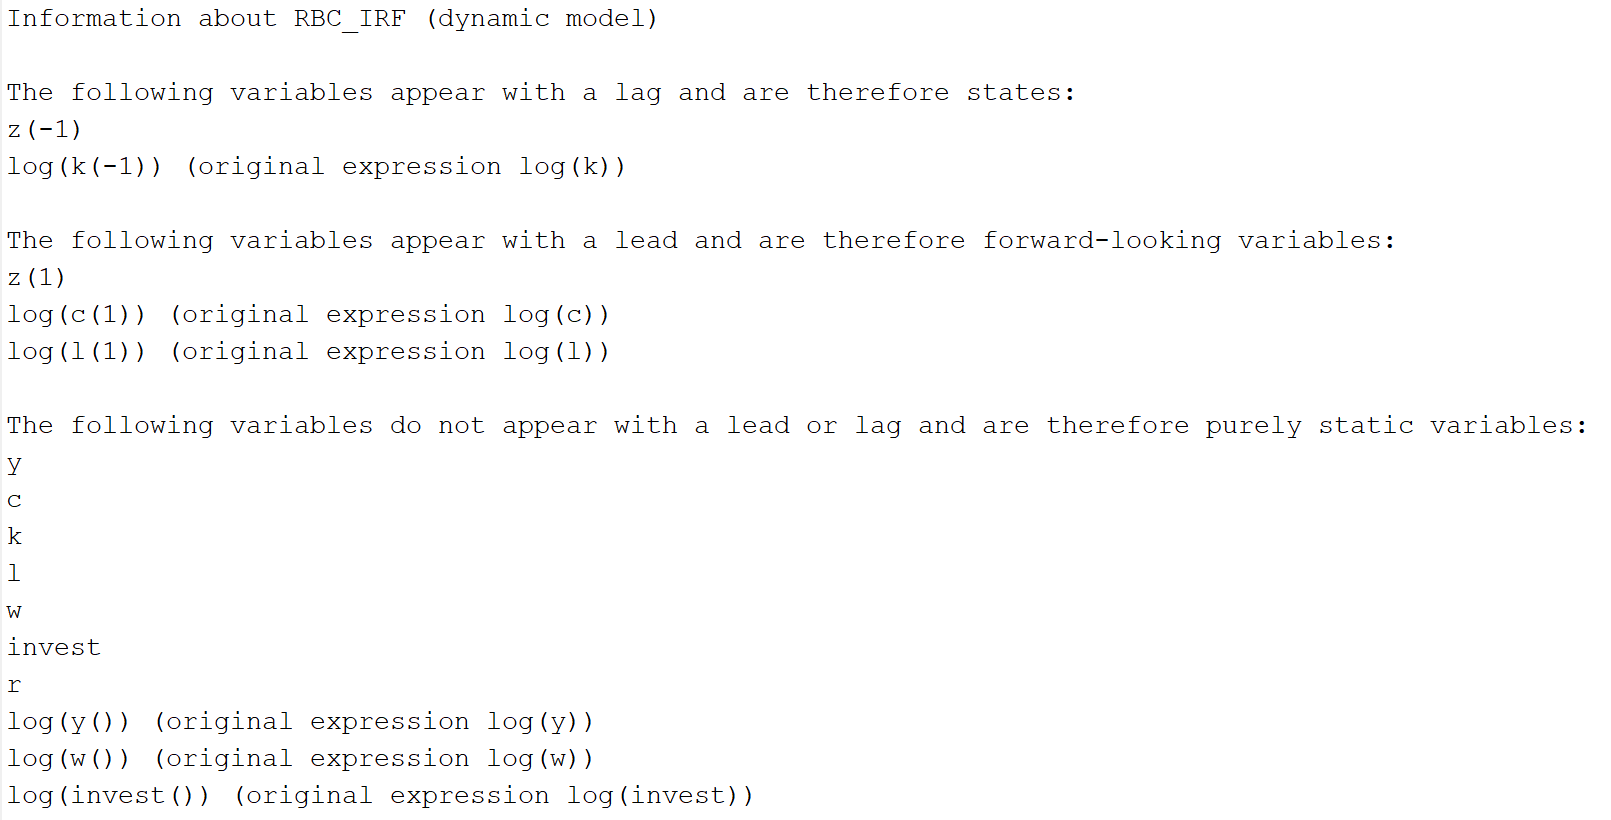
\includegraphics[width=11cm]{figures/RBC_model_info}
\end{figure}
\end{frame}


\begin{frame}[fragile]{Checking Blanchard/Kahn conditions}{\texttt{RBC\_IRF.mod}}
\begin{itemize}
\item To check the Blanchard/Kahn conditions, use
\begin{minted}{c++}
check;
\end{minted}
\end{itemize}
\begin{figure}
\center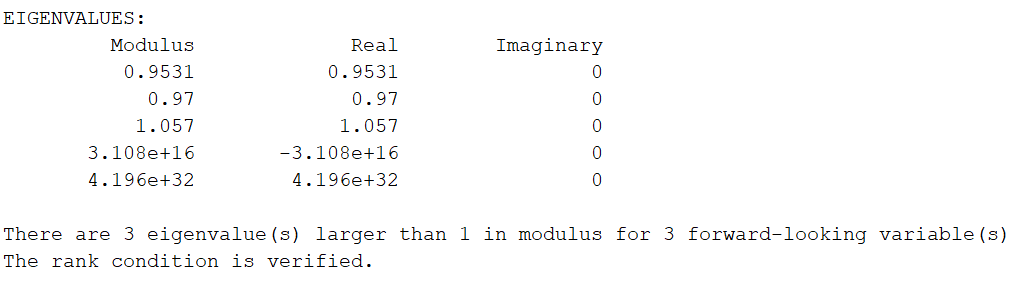
\includegraphics[width=11cm]{figures/RBC_check}
\end{figure}
\end{frame}


\renewcommand{\Source}{\textcite{DejongDave2011}, Ch.\ 4.3}


\subsection{\thesection.\thesubsection \ Solution via Eigenvalue Decomposition}

\begin{frame}{Solving the system: Eigenvalue decomposition}
\begin{small}
\begin{itemize}
\item Recall that $a_t$ in \eqref{sys_inverted} contains two state (backward-looking) variables: $x_t \equiv [ \begin{array}{ccc} \hat{k}_{t-1} & {z}_t \end{array} ]' $ and one control (forward-looking) variable $u_t = \hat{c}_t$
\item Decouple the system using an \highlight{Eigenvalue (Jordan) decomposition}:
\begin{equation}
W = D \Lambda D^{-1}\: ,
\end{equation}
where matrix $\Lambda$ has eigenvalues on its main diagonal and $D$ is a matrix of eigenvectors
\item Then system \eqref{sys_inverted}, $\mathbb{E}_t a_{t+1} = W a_t$, can be rewritten as
\begin{align} \notag
           \mathbb{E}_t \underbrace{D^{-1} a_{t+1}}_{\equiv \zeta_{t+1}} &= \Lambda \underbrace{D^{-1} a_{t}}_{\equiv \zeta_t} \\ \label{decomposed}
    \mathbb{E}_t \zeta_{t+1}&=\Lambda \zeta_t
          \end{align}
\item This yields a set of independent univariate difference equations in $\zeta_{i,t}$
\begin{align*}
  \mathbb{E}_t \zeta_{1,t+1} &= \lambda_1 \zeta_{1,t}  \\
   &\vdots  \\
  \mathbb{E}_t \zeta_{i,t+1} &= \lambda_i \zeta_{i,t}
\end{align*}
\end{itemize}
\end{small}
\end{frame}

\begin{frame}{Solving the system: Reordering}
\begin{witemize}
\item Elements in $\Lambda$ can be ordered in ascending order without loss of generality (note: we need to reshuffle the eigenvectors accordingly)
\item Assume that number of explosive eigenvalues equal to $n_u$ and partition reordered $D$ and $\Lambda$ and matrix $W$ according to stable and explosive eigenvalues
\footnotesize{
\[ \Lambda = \left[\begin{array}{cc}
               \underset{n_x\times n_x}{\Lambda_1} & \underset{n_x \times n_u}{0} \\
               \underset{n_u\times n_x}{0} & \underset{ n_u \times n_u}{\Lambda_2}
             \end{array} \right]; W=  \left[\begin{array}{cc}
               \underset{n_x\times n_x}{w_{11}} & \underset{n_x\times n_u}{w_{12}} \\
               \underset{n_u\times n_x}{w_{21}} & \underset{n_u\times n_u}{w_{22}}
             \end{array} \right]; D^{-1}=  \left[\begin{array}{cc}
               \underset{n_x\times n_x}{q_{11}} & \underset{n_x\times n_u}{q_{12}} \\
               \underset{n_u\times n_x}{q_{21}} & \underset{n_u\times n_u}{q_{22}}
             \end{array} \right] \]}
\item Also partition $\zeta_t=\left[\begin{array}{cc}
                         \underset{1 \times n_x}{\zeta_{1,t}} & \underset{1 \times n_u}{\zeta_{2,t}}
                       \end{array}
 \right]'$
\end{witemize}
\end{frame}


\begin{frame}{Solving the system: Solution for controls}
\begin{itemize}
\item First, consider the lower part of \eqref{decomposed} corresponding to controls: $ \mathbb{E}_t \zeta_{2,t+1}=\Lambda_2 \zeta_{2,t}$
\item As in the univariate case, this part is iterated forward
\begin{equation}
 \zeta_{2,t}=\lim_{k \rightarrow \infty} \Lambda_2^{-k} \mathbb{E}_t \zeta_{2,t+k}  = 0,
\end{equation}
as the diagonal elements of $\Lambda_2$ are explosive and $\lim_{t \rightarrow \infty} = |\zeta_{2,t}| < \infty$ (linear combination of bounded variables)
\item From the definition of $\zeta_t$ follows
\begin{equation}
 \left[ \begin{array}{c}
                \underset{n_x \times 1}{\zeta_{1,t}} \\
               \underset{n_u \times 1}{\zeta_{2,t}}
               \end{array} \right] =
               \underbrace{\left[\begin{array}{cc}
               \underset{n_x\times n_x}{q_{11}} & \underset{n_x\times n_u}{q_{12}} \\
               \underset{n_u\times n_x}{q_{21}} & \underset{n_u\times n_u}{q_{22}} \end{array} \right]}_{D^{-1}}
                 \underbrace{\left[  \begin{array}{c}
                                              \widehat{x}_t \\
                                              \widehat{u}_t
                                            \end{array}\right]}_{a_t}
\end{equation}
\item Using $ \zeta_{2,t}=0$ implies we have a linear policy function for the controls:
\begin{equation}\label{policy solution}
  0 = {q_{21}}{{\hat x}_t} + {q_{22}}{{\hat u}_t} \Rightarrow \widehat{u}_t = \underbrace{-q_{22}^{-1}q_{21} }_{\equiv M} \widehat{x}_t
\end{equation}
\end{itemize}
\end{frame}


\begin{frame}{Solving the system: Solution for states I}
\begin{itemize}
    \item Given the partitioning of $W$, the upper part of
    \begin{equation}  \tag{\ref{sys_inverted}}
    \mathbb{E}_t a_{t+1} =\underbrace{A^{-1}B}_{\equiv W}a_t
\end{equation}
is given
    \begin{equation}
    \mathbb{E}_t \widehat{x}_{t+1}=w_{11} \widehat{x}_t+w_{12} \widehat{u}_t,
    \end{equation}
    \item Substituting for $\widehat{u}_t$ using
    \begin{equation}\tag{\ref{policy solution}'}
  \widehat{u}_t = \underbrace{-q_{22}^{-1}q_{21} }_{\equiv H} \widehat{x}_t=H\widehat{x}_t
\end{equation}
 gives
    \begin{equation}
        \mathbb{E}_t \widehat{x}_{t+1}=\underbrace{(w_{11}-w_{12}q_{22}^{-1}q_{21})}_{\equiv F} \widehat{x}_t
    \end{equation}
\end{itemize}
\end{frame}

\begin{frame}{Solving the system: Solution for states II}
\begin{itemize}
   \item Denote the number of endogenous states with $n_{x1}$ and of the exogenous states with $n_{x2}$
    \item With endogenous state variables being predetermined
    \begin{equation}
    \widehat{x}^1_{t} = \mathbb{E}_t \widehat{x}^1_{t}
    \end{equation}
    and given the exogenous LOM
    \begin{equation}\tag{\ref{eq: shocks}}
    x_{t}^2 = \Gamma x_{t-1}^2 + \epsilon_{t} \: ,
    \end{equation}
 we have
    \begin{equation}\label{actual law of motion solution}
       \widehat{x}_{t+1}=\mathbb{E}_t\widehat{x}_{t+1} + \underbrace{\left[ \begin{array}{c}
                                     0_{n_{x_1} \times n_{x_2}} \\
                                     I_{n_{x_2} \times n_{x_2}}
                                   \end{array}
     \right]}_{\equiv \eta} \epsilon_{t+1} = F \widehat{x}_t + \eta  \epsilon_{t+1}
    \end{equation}
\end{itemize}
\end{frame}

\begin{frame}{The solution}
\begin{itemize}
    \item Taken together, the solution equations \eqref{policy solution} and \eqref{actual law of motion solution} provide a recursive representation of the solution to \eqref{ABform} in \highlight{state space form}:
    \begin{align}
      \widehat{u}_t  &= H \widehat{x}_t\\
         \widehat{x}_{t+1}&= F \widehat{x}_t + \eta  \epsilon_{t+1}
    \end{align}
    \item The first equation is called \highlight{observation equation} or \highlight{measurement equation}, while the second one is called \highlight{state transition equation}
\end{itemize}
\end{frame}

\section{Dynare implementation}
\begin{frame}{Solution storage in Dynare}
\begin{itemize}
    \item Note that Dynare internally stacks controls and states into one equation:
    \begin{equation}
      y_t=y + gh_x (x_{t-1}-x)+gh_u\epsilon_t
    \end{equation}
    where \texttt{ghx} and \texttt{ghu} are subfields of \texttt{oo\_.dr}
    \begin{figure}
      \centering
      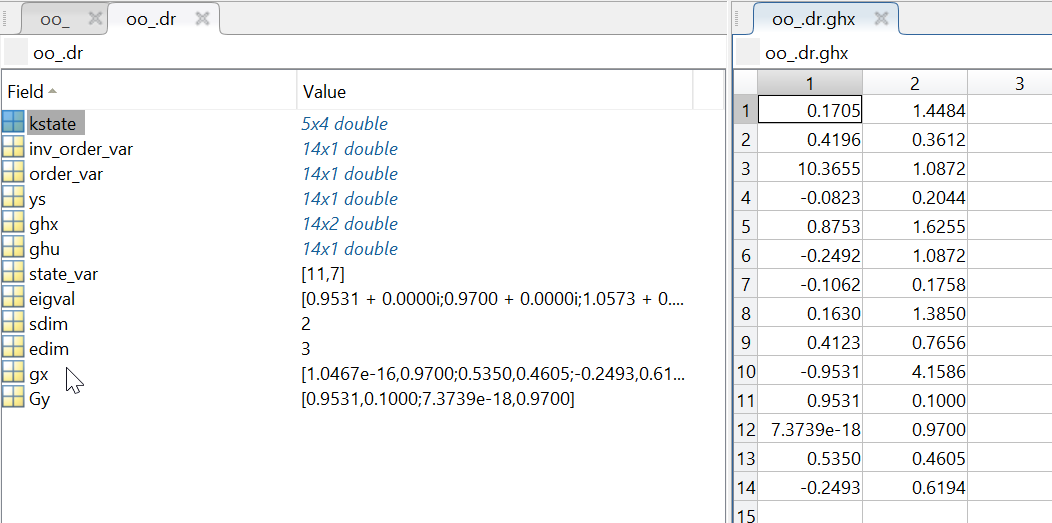
\includegraphics[width=9cm]{figures/RBC_oo_DR}
    \end{figure}
\end{itemize}
\end{frame}

\begin{frame}[fragile]{Decision rules in Dynare}{\texttt{RBC\_IRF.mod}}
\begin{itemize}
    \item Dynare will display the decision rules in digestible form at \texttt{order<3}
    \begin{minted}{c++}
    stoch_simul(order=1);
    \end{minted}
\begin{figure}
  \centering
  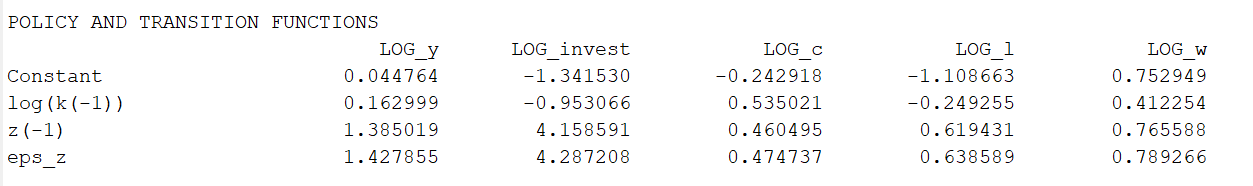
\includegraphics[width=11cm]{figures/RBC_DR}
\end{figure}
    \item The results are stored in \texttt{oo\_.dr}
\end{itemize}

\end{frame}


\begin{frame}[fragile]{Making use of the solution}{\texttt{RBC\_baseline.mod}}
\begin{itemize}
    \item Well-established techniques for linear state space solutions allow computation of theoretical moments, even with linear filters, and of (conditional) variance decompositions
    \begin{minted}{c++}
stoch_simul(order=1,irf=20,conditional_variance_decomposition=[1,4]);
stoch_simul(order=1,hp_filter=1600);
    \end{minted}
    \item Given $x_0$, state-space solution can be used to simulate equilibrium time series for given sequence $\{ \epsilon_{t}\}_{t = 0}^\infty $\\
        $\rightarrow$ allows computation of simulated moments, impulse responses, conditional and unconditional forecasts
    \begin{minted}{c++}
stoch_simul(order=1,irf=20,periods=1000,drop=200);
    \end{minted}
    \item At \texttt{order=1}, IRFs are invariant to the point in the state space\\
    $\rightarrow$ only one simulation necessary
\end{itemize}
\end{frame}

\begin{frame}[fragile]{RBC Output}
\begin{figure}
  \centering
  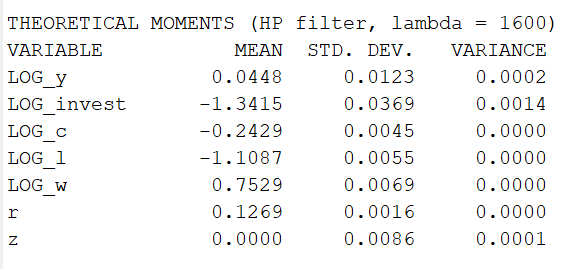
\includegraphics[width=7cm]{figures/RBC_moments}\includegraphics[width=7cm]{Codes/RBC_IRF/graphs/RBC_IRF_IRF_eps_z}
\end{figure}

\end{frame}

\begin{frame}[fragile]{RBC Output with government spending shocks}
\begin{figure}
  \centering
  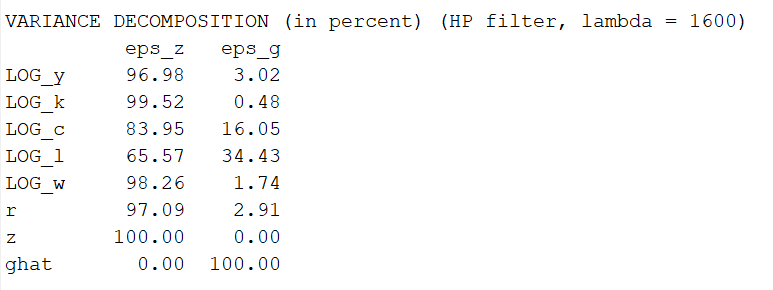
\includegraphics[width=8cm]{figures/RBC_G_var_decomp.png}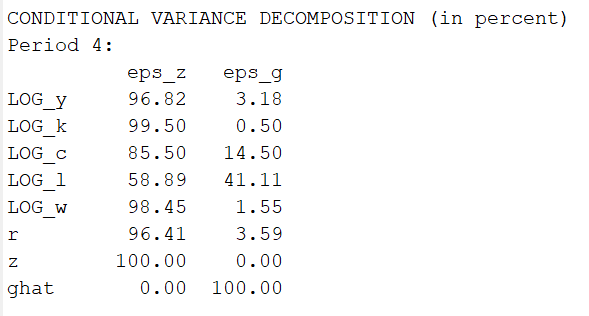
\includegraphics[width=6cm]{figures/RBC_G_cond_var_decomp.png}
\end{figure}

\end{frame}


\renewcommand{\Source}{}

\part{References}

\begin{frame}[allowframebreaks]{Bibliography}
\printbibliography
\end{frame}


\end{document}
